\section{Bestrahlungsplanung}
\label{sec:Bestrahlungsplanung}

Bevor mit der Planung der Bestrahlung begonnen werden kann, wird zunächst die Kontur des Körpers in dem Contouring Programm eingezeichnet.
Es wird außerdem die Kontur von der Lunge eingezeichnet, da sich diese in unmittelbarer nähe zu dem PTV befindet.
Um die gewünschte Dosisverteilung in der Schulter zu erreichen, wird die Planung mit zwei opponierenden Feldern durchgeführt.
Diese Felder sind gleich groß und haben die Größen $\SI{10.5}{\centi\meter}$ x $\SI{9}{\centi\meter}$. Diese Felder haben eine Gantry Position von
$0°$ und $180°$. Damit das umliegende Gewebe geschützt wird, werden außerdem MLCs mit den beiden Feldern Verwendet. Die Einstellungen der MLCs sind
in der Abbildung \ref{abb:MLC} dargestellt. Bei diesem Plan sind die beiden Felder nicht gleich Gewichtet, sondern das erste Feld, bei $0°$, ist $60\%$
gewichtet und das zweite Feld, bei $180°$, ist $40\%$ gewichtet. Der Plan ist auf \enquote{$100\%$ target mean} normiert worden.

\begin{figure}[H]
  \centering
  \begin{subfigure}{\textwidth}
    \centering
    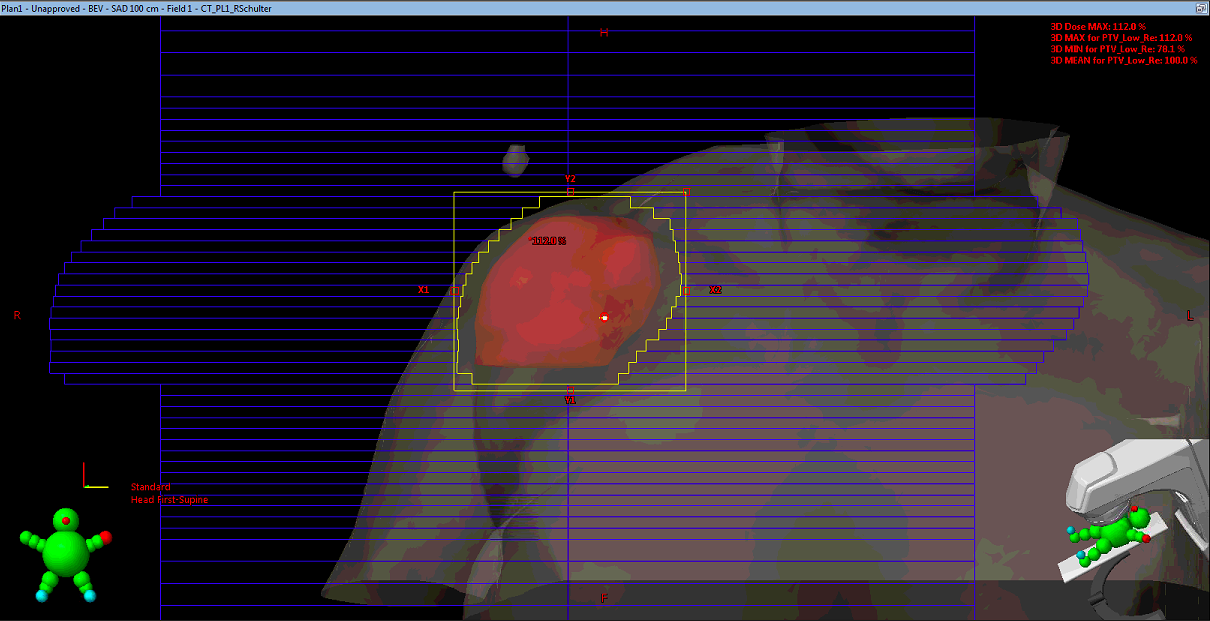
\includegraphics[height = 5cm]{Bilder/MLC_Schulter1.png}
    \caption{}
  \end{subfigure}
  \begin{subfigure}{\textwidth}
    \centering
    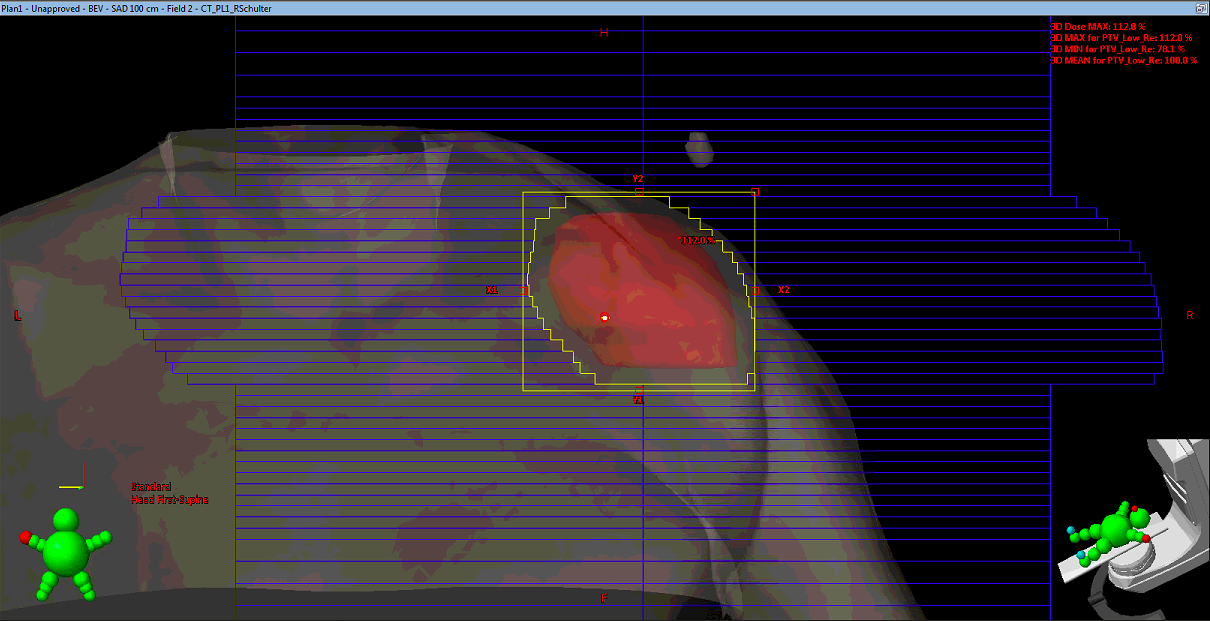
\includegraphics[height=5cm]{Bilder/MLC_Schulter2.png}
    \caption{}
  \end{subfigure}
  \caption{Darstellung der Lamellenpositionen der beiden Felder. Bei a) die Positionen bei dem Feld bei $0°$ und bei b) die Positionen bei dem Feld bei $180°$.}
  \label{abb:MLC}
\end{figure}
